\clearpage
\section{Classification multi-classes}

Dans cette partie nous allons appliqué une regression logistique \textit{One-Vs-All} dans l'objectif de prédire la valeur numérique d'un chiffre manuscrit. \\

\noindent
Le procéder est assez simple, comme le montre la figure \ref{fig:multi-class-scheme}:

\begin{figure}[!h]
    \begin{minipage}{.48\linewidth}
        Nous avons au total 3 classes, on prend une classe et on l'isole des deux autres.
        Ce qui nous en donne 2, avec lesquels nous allons réaliser une regression logistique. Si on réalise 3 fois cette étapes alors nous aurons 3 limites de décision. \\
        Dans le cas d'une prédiction, nous allons pouvoir calculer les probabilités pour lesquelles notre échantillon se trouve dans une des limites de décision grâce à notre modèle. La probabilité
        la plus importante nous permettra de déterminer dans qu'elle classe ce trouve notre chiffre manuscrit.

        \begin{equation}\label{eq:proba-multi}
            h_{\theta}^{(i)} = P(y=i|x;\theta) \quad (i = 1, 2, 3)
         \end{equation}

    \end{minipage}\hfill
    \begin{minipage}{.48\linewidth}
        \begin{center}
            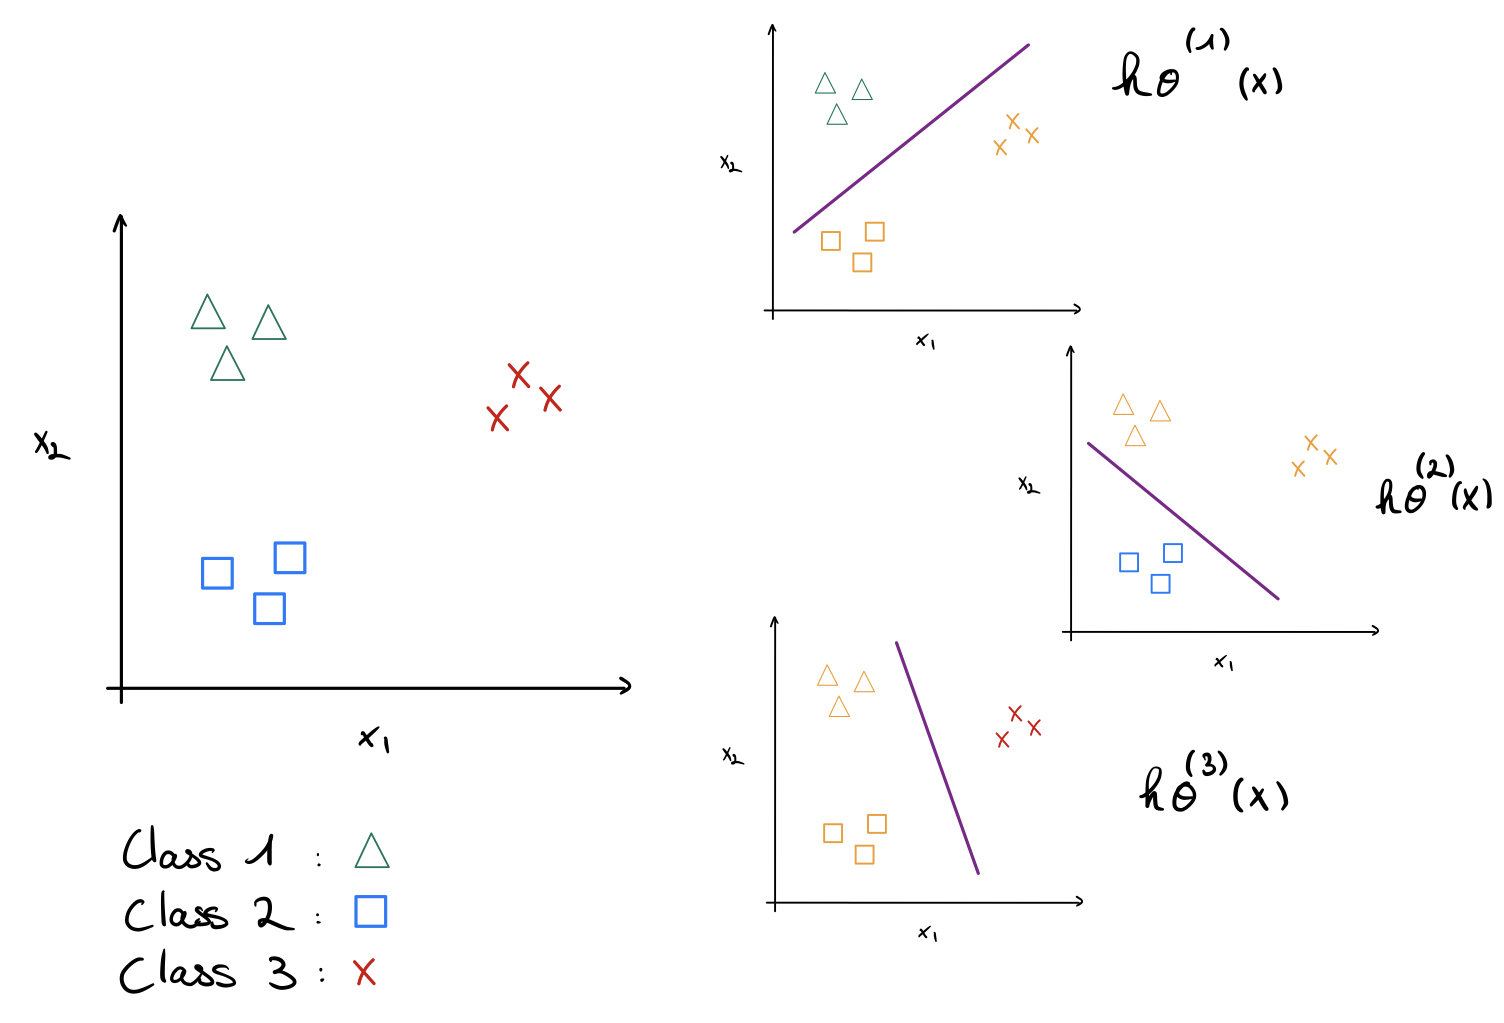
\includegraphics[width=1\textwidth]{./img/multi-class-scheme.jpeg}
            \caption{\label{fig:multi-class-scheme}Schéma explicatif de la classification multi-classes}  
        \end{center}
    \end{minipage}
\end{figure}

\noindent
Dans notre cas nous n'aurons pas 3 classes mais 10, il faudra donc réaliser 10 classifieur.

\subsection{Visualisation des données}

Dans notre matrice $X$ nous avons 5000 échantillon de chiffre manuscrit, où chaque ligne représente une image d'un chiffre en niveau de gris de $20x20$px. Ce qui nous donne finalement une matrice de dimension 
5000 sur 400. \\
Nous allons en afficher une centaine de manière aléatoire à l'aide du script données. Chaque visualisation est différente.

\begin{figure}[!h]
    \begin{center}
        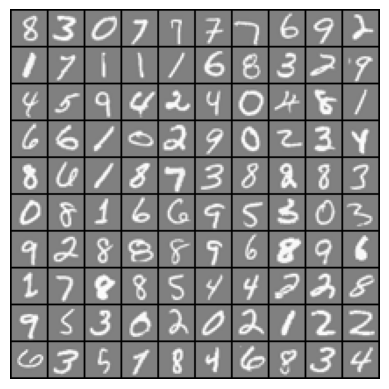
\includegraphics[width=0.4\textwidth]{./img/5.2.png}
        \caption{\label{fig:5.2}Visualisation des données}  
    \end{center}
\end{figure}

\clearpage
\subsection{Véctorisation de la régression logistique}

Pour cette partie il est important que notre régression logistique soit vectorisé, notre échantilllon de données est important comparé aux exercices précédents. \\
La vectorisation a de nombreux avantages:

\begin{enumerate}
    \item Apprentissage plus rapide
    \item Code plus lisible
    \item Moins d'erreur lié au boucle
    \item ...
\end{enumerate}

\subsubsection{Vectorisation de la fonction de coût $J(\theta)$}

Grâce à python et aux fonctions de numpy la vectorisation s'applique facilement. Il faut coder la fonction de coût comme elle est écrite en retirant les $^{(i)}$ lié à la somme et en la remplacant par \textit{np.sum()}. \\
La fonction de coût est alors réduite à une ligne, grâce aux multiplications matricielles automatique de python et numpy.

\begin{equation}\label{eq:cout}
    J(\theta) = \frac{1}{m} \sum_{i=0}^{m-1}[-y^{(i)} log(h_\theta(x^{(i)})) - (1-y^{(i)}) log(1-h_\theta(x^{(i)}))]
\end{equation}

\begin{figure}[!h]
\begin{minted}[frame=lines, framesep=2mm, baselinestretch=1.2, fontsize=\footnotesize, linenos, breaklines=true]{python}
def lrCostFunction(theta, X, y, Lambda):
    theta = theta.reshape((n,1)) # (4,1)
 
    h = sigmoid(X @ theta)
    J = (1/m) * np.sum(-y * np.log(h) - (1 - y) * np.log(1 - h))
      
    return J
\end{minted}   
\captionof{listing}{Fonction de coût vectorisé}
\end{figure}

\subsubsection{Vectorisation de la descente de gradient}
\noindent
Le principe est le même que pour la fonction de coût $J(\theta)$:

\begin{equation}\label{eq:descente-gradient}
    \frac{\partial J(\theta)}{\partial \theta_j} = \frac{1}{m} \sum_{i=0}^{m} (h_\theta(x^{(i)}) - y^{(i)}) x_j^{(i)}
\end{equation}

\begin{figure}[!h]
\begin{minted}[frame=lines, framesep=2mm, baselinestretch=1.2, fontsize=\footnotesize, linenos, breaklines=true]{python}
def lrCostGradient(theta, X, y, Lambda):
    theta = theta.reshape((n,1)) # (4,1)

    h = sigmoid(X @ theta)
    grad = (1/m) * (X.T @ (h - y))

    return grad.flatten()
\end{minted}   
\captionof{listing}{Descente de gradient vectorisé}
\end{figure}


\subsubsection{Application d'une régulation}

Comme expliqué plus tôt la régulation permet d'éviter le problème d'\textit{overfit} si $\lambda$ est correctement choisis. Dans ce problème nous avons un nombre important de caratéristiques, il est
donc important de réaliser une régulation.

\vspace{0.4cm}
\noindent
\textbf{Fonction de coût régularisé et vectorisé}

\begin{equation}\label{eq:cout-reg}
    J(\theta) = \frac{1}{m} \sum_{i=0}^{m-1}[-y^{(i)} log(h_\theta(x^{(i)})) - (1-y^{(i)}) log(1-h_\theta(x^{(i)}))] + \frac{\lambda}{2m} \sum_{j=1}^{n-1} \theta_j^2
\end{equation}

\begin{figure}[!h]
\begin{minted}[frame=lines, framesep=2mm, baselinestretch=1.2, fontsize=\footnotesize, linenos, breaklines=true]{python}
def lrCostFunction(theta, X, y, Lambda):
    theta = theta.reshape((n,1)) # (4,1)
    h = sigmoid(X @ theta)
    J = (1/m) * np.sum(-y * np.log(h) - (1 - y) * np.log(1 - h)) + ((Lambda/(2*m)) * np.sum(theta[1:]**2)) #conventionnellement on n'applique pas la reg sur theta0 d'où theta[1:]
        
    return J

    """return 
    Cost: 0.734819
    Expected cost: 0.734819
    """
\end{minted}   
\captionof{listing}{Fonction de coût régularisé et vectorisé}
\end{figure}


\vspace{0.4cm}
\noindent
\textbf{Descente de gradient régularisé et vectorisé}

\begin{align}\label{eq:descente-gradient-reg}
    \frac{\partial J(\theta)}{\partial \theta_j} = \frac{1}{m} \sum_{i=0}^{m} (h_\theta(x^{(i)}) - y^{(i)}) x_j^{(i)} \qquad \qquad \qquad \text{pour} \quad j=0 \\
    \frac{\partial J(\theta)}{\partial \theta_j} = \frac{1}{m} \left( \sum_{i=0}^{m} (h_\theta(x^{(i)}) - y^{(i)}) x_j^{(i)} + \lambda \theta_j \right) \qquad \qquad \qquad \text{pour} \quad j\geq1 
\end{align}

\begin{figure}[!h]
\begin{minted}[frame=lines, framesep=2mm, baselinestretch=1.2, fontsize=\footnotesize, linenos, breaklines=true]{python}
def lrCostGradient(theta, X, y, Lambda):
    theta = theta.reshape((n,1)) # (4,1)
    h = sigmoid(X @ theta)
    grad = (1/m) * (X.T @ (h - y))
    grad[1:] += (Lambda/m * theta[1:]) # reg pour j >= 1 (comme pour J(theta)) et theta != 0 (conventionnellement)

    return grad.flatten()

    """return 
    Gradients:[0.14656137 0.05144159 0.12472227 0.19800296]
    Expected gradients: 0.14656137  0.05144159  0.12472227  0.19800296
    """
\end{minted}   
\captionof{listing}{Descente de gradient régularisé et vectorisé}
\end{figure}

\clearpage
\subsection{Apprentissage d'un classifieur One-Vs-All}

Pour réaliser ce classifieur nous avons 10 classes, il nous faut donc 10 étiquettes. Il faut calculer les theta pour chaque classe pour cela on utilise un vecteur d'etiquette de dimension 10 indiquant 
la classe actuel. Par la suite à l'aide l'algorithme d'optimisation \textit{fmin\_tnc} on minimise les theta pour l'étiquette \textit{(la classe)} correspondante puis on les stocks avant de passer à la 
classe suivante.

\begin{figure}[!h]
\begin{minted}[frame=lines, framesep=2mm, baselinestretch=1.2, fontsize=\footnotesize, linenos, breaklines=true]{python}
def learnOneVsAll(X, y, num_labels, Lambda):
    m, n = X.shape
    all_theta = np.zeros((num_labels, n))
    initial_theta = np.zeros((n, 1))

    for i in range(1,num_labels+1):
        print('Optimizing for handwritten number %d...' %i)
        y_1vsAll = (y == i)*1

        result = fmin_tnc(lrCostFunction, fprime=lrCostGradient, x0=initial_theta, args=(X, y_1vsAll, Lambda), disp=False)
        
        all_theta[i-1,:] = result[0]

    return all_theta
\end{minted}   
\captionof{listing}{Apprentissage du classifieur}
\end{figure}
        

\subsection{Prédiction One-Vs-All}

La fonction \textit{predictOneVsAll} nous permet de prédire le chiffre manuscrit grâce à classifieur, cette prédiction est réalisé pour tous les chiffres de X, 5000 au total. \\
Notre classifieur nous permet d'obtenir une prédiction de $96.46\%$, ce qui est plus que satifaisant sur un total de 5000 chiffres.\\


Pour ce faire on calcul la probabilité que le chiffre $X[i]$ appartient à l'une des 10 classes, ce qui nous donne 10 probabilités. On prends alors la plus grande, ce qui nous donne le chiffre numérique
correspondant.

\begin{figure}[!h]
\begin{minted}[frame=lines, framesep=2mm, baselinestretch=1.2, fontsize=\footnotesize, linenos, breaklines=true]{python}
def predictOneVsAll(all_theta, X):
    m = X.shape[0]
    p = np.zeros((m, 1))
    p = np.argmax(sigmoid(X @ all_theta.T), axis=1) + 1

    return p
\end{minted}   
\captionof{listing}{Prédiction One-Vs-All}
\end{figure}
